% Options for packages loaded elsewhere
\PassOptionsToPackage{unicode}{hyperref}
\PassOptionsToPackage{hyphens}{url}
\PassOptionsToPackage{dvipsnames,svgnames,x11names}{xcolor}
%
\documentclass[
  letterpaper,
  DIV=11,
  numbers=noendperiod]{scrartcl}

\usepackage{amsmath,amssymb}
\usepackage{iftex}
\ifPDFTeX
  \usepackage[T1]{fontenc}
  \usepackage[utf8]{inputenc}
  \usepackage{textcomp} % provide euro and other symbols
\else % if luatex or xetex
  \usepackage{unicode-math}
  \defaultfontfeatures{Scale=MatchLowercase}
  \defaultfontfeatures[\rmfamily]{Ligatures=TeX,Scale=1}
\fi
\usepackage{lmodern}
\ifPDFTeX\else  
    % xetex/luatex font selection
\fi
% Use upquote if available, for straight quotes in verbatim environments
\IfFileExists{upquote.sty}{\usepackage{upquote}}{}
\IfFileExists{microtype.sty}{% use microtype if available
  \usepackage[]{microtype}
  \UseMicrotypeSet[protrusion]{basicmath} % disable protrusion for tt fonts
}{}
\makeatletter
\@ifundefined{KOMAClassName}{% if non-KOMA class
  \IfFileExists{parskip.sty}{%
    \usepackage{parskip}
  }{% else
    \setlength{\parindent}{0pt}
    \setlength{\parskip}{6pt plus 2pt minus 1pt}}
}{% if KOMA class
  \KOMAoptions{parskip=half}}
\makeatother
\usepackage{xcolor}
\setlength{\emergencystretch}{3em} % prevent overfull lines
\setcounter{secnumdepth}{-\maxdimen} % remove section numbering
% Make \paragraph and \subparagraph free-standing
\ifx\paragraph\undefined\else
  \let\oldparagraph\paragraph
  \renewcommand{\paragraph}[1]{\oldparagraph{#1}\mbox{}}
\fi
\ifx\subparagraph\undefined\else
  \let\oldsubparagraph\subparagraph
  \renewcommand{\subparagraph}[1]{\oldsubparagraph{#1}\mbox{}}
\fi


\providecommand{\tightlist}{%
  \setlength{\itemsep}{0pt}\setlength{\parskip}{0pt}}\usepackage{longtable,booktabs,array}
\usepackage{calc} % for calculating minipage widths
% Correct order of tables after \paragraph or \subparagraph
\usepackage{etoolbox}
\makeatletter
\patchcmd\longtable{\par}{\if@noskipsec\mbox{}\fi\par}{}{}
\makeatother
% Allow footnotes in longtable head/foot
\IfFileExists{footnotehyper.sty}{\usepackage{footnotehyper}}{\usepackage{footnote}}
\makesavenoteenv{longtable}
\usepackage{graphicx}
\makeatletter
\def\maxwidth{\ifdim\Gin@nat@width>\linewidth\linewidth\else\Gin@nat@width\fi}
\def\maxheight{\ifdim\Gin@nat@height>\textheight\textheight\else\Gin@nat@height\fi}
\makeatother
% Scale images if necessary, so that they will not overflow the page
% margins by default, and it is still possible to overwrite the defaults
% using explicit options in \includegraphics[width, height, ...]{}
\setkeys{Gin}{width=\maxwidth,height=\maxheight,keepaspectratio}
% Set default figure placement to htbp
\makeatletter
\def\fps@figure{htbp}
\makeatother
% definitions for citeproc citations
\NewDocumentCommand\citeproctext{}{}
\NewDocumentCommand\citeproc{mm}{%
  \begingroup\def\citeproctext{#2}\cite{#1}\endgroup}
\makeatletter
 % allow citations to break across lines
 \let\@cite@ofmt\@firstofone
 % avoid brackets around text for \cite:
 \def\@biblabel#1{}
 \def\@cite#1#2{{#1\if@tempswa , #2\fi}}
\makeatother
\newlength{\cslhangindent}
\setlength{\cslhangindent}{1.5em}
\newlength{\csllabelwidth}
\setlength{\csllabelwidth}{3em}
\newenvironment{CSLReferences}[2] % #1 hanging-indent, #2 entry-spacing
 {\begin{list}{}{%
  \setlength{\itemindent}{0pt}
  \setlength{\leftmargin}{0pt}
  \setlength{\parsep}{0pt}
  % turn on hanging indent if param 1 is 1
  \ifodd #1
   \setlength{\leftmargin}{\cslhangindent}
   \setlength{\itemindent}{-1\cslhangindent}
  \fi
  % set entry spacing
  \setlength{\itemsep}{#2\baselineskip}}}
 {\end{list}}
\usepackage{calc}
\newcommand{\CSLBlock}[1]{\hfill\break\parbox[t]{\linewidth}{\strut\ignorespaces#1\strut}}
\newcommand{\CSLLeftMargin}[1]{\parbox[t]{\csllabelwidth}{\strut#1\strut}}
\newcommand{\CSLRightInline}[1]{\parbox[t]{\linewidth - \csllabelwidth}{\strut#1\strut}}
\newcommand{\CSLIndent}[1]{\hspace{\cslhangindent}#1}

\KOMAoption{captions}{tableheading}
\makeatletter
\@ifpackageloaded{caption}{}{\usepackage{caption}}
\AtBeginDocument{%
\ifdefined\contentsname
  \renewcommand*\contentsname{Table of contents}
\else
  \newcommand\contentsname{Table of contents}
\fi
\ifdefined\listfigurename
  \renewcommand*\listfigurename{List of Figures}
\else
  \newcommand\listfigurename{List of Figures}
\fi
\ifdefined\listtablename
  \renewcommand*\listtablename{List of Tables}
\else
  \newcommand\listtablename{List of Tables}
\fi
\ifdefined\figurename
  \renewcommand*\figurename{Figure}
\else
  \newcommand\figurename{Figure}
\fi
\ifdefined\tablename
  \renewcommand*\tablename{Table}
\else
  \newcommand\tablename{Table}
\fi
}
\@ifpackageloaded{float}{}{\usepackage{float}}
\floatstyle{ruled}
\@ifundefined{c@chapter}{\newfloat{codelisting}{h}{lop}}{\newfloat{codelisting}{h}{lop}[chapter]}
\floatname{codelisting}{Listing}
\newcommand*\listoflistings{\listof{codelisting}{List of Listings}}
\makeatother
\makeatletter
\makeatother
\makeatletter
\@ifpackageloaded{caption}{}{\usepackage{caption}}
\@ifpackageloaded{subcaption}{}{\usepackage{subcaption}}
\makeatother
\ifLuaTeX
  \usepackage{selnolig}  % disable illegal ligatures
\fi
\usepackage{bookmark}

\IfFileExists{xurl.sty}{\usepackage{xurl}}{} % add URL line breaks if available
\urlstyle{same} % disable monospaced font for URLs
\hypersetup{
  pdftitle={Quarto-manuscript01},
  colorlinks=true,
  linkcolor={blue},
  filecolor={Maroon},
  citecolor={Blue},
  urlcolor={Blue},
  pdfcreator={LaTeX via pandoc}}

\title{Quarto-manuscript01}
\usepackage{etoolbox}
\makeatletter
\providecommand{\subtitle}[1]{% add subtitle to \maketitle
  \apptocmd{\@title}{\par {\large #1 \par}}{}{}
}
\makeatother
\subtitle{Reproduction}
\author{Robert C. Cline, Sr.}
\date{}

\begin{document}
\maketitle

\subsection{Quarto manuscripts:
https://quarto.org/docs/manuscripts}\label{quarto-manuscripts-httpsquarto.orgdocsmanuscripts}

\subsubsection{Slides}\label{slides}

\begin{itemize}
\tightlist
\item
  mine.quarto.pub/quarto-manuscdripts-rmed\\
\item
  github.com/mine-cetinkaya-rundel/quarto-manuscrpts-rmed
\end{itemize}

\subsubsection{Manuscript:}\label{manuscript}

\begin{itemize}
\tightlist
\item
  mine-cetinkaya-rundel.github.io/indo-rct\\
\item
  github.com/mine-cetinkaya-rundel/indo-rct
\end{itemize}

\subsection{Section}\label{section}

This is a simple placeholder for the manuscript's main document (Knuth
1984). Mine Certinkaya-Rundel presented a webinar on the steps to create
a Quarto-Manuscript on March 24, 2024 (R Consortium 2024)\footnote{C.f.
  YouTube presentation
  \emph{https://www.youtube.com/watch?v=NK1onTLcgY4\&t=1265s}}

\subsection{Study outcomes}\label{study-outcomes}

\begin{figure}[H]

\centering{

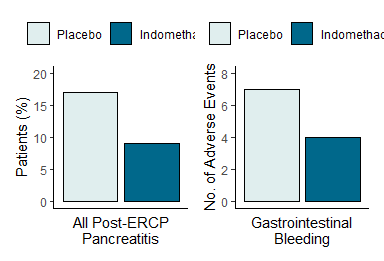
\includegraphics{index_files/figure-latex/notebooks-incidences-fig-incidences-adverse-events-output-1.png}

}

\caption{\label{fig-incidences-adverse-events}Incidence of the Primary
and Secondary End Points and Adverse Events}

\end{figure}%

\textsubscript{Source:
\href{https://rccline.github.io/quarto-manuscript01/notebooks/incidences-preview.html\#cell-fig-incidences-adverse-events}{Incidence}}

\textsubscript{Source:
\href{https://rccline.github.io/quarto-manuscript01/index.qmd.html}{Article
Notebook}}

\textbf{This is an example of inline code}:\\
The mean body mass of penguins is 4201.75 grams.\\
What if we use a label ((\textbf{penguin\_bodymass?}))

\textbf{Cross-referencing}

\begin{itemize}
\tightlist
\item
  This is a cross-reference to our
  (Figure~\ref{fig-incidences-adverse-events}).\\
\item
  You can also bring up the \emph{cross-reference-insert-anything tool}
  by typing:
\end{itemize}

\subsection{Citations}\label{citations}

In Visual mode: Insert citation or, control-shift-F8 (Hennekens et al.
1996)

This is a sample citation from a paper published in 2012 which you can
find at: https://pubmed.ncbi.nlm.nih.gov/8929364/ DOI:
10.1056/NEJM199611283352207

Reference for (Figure~\ref{fig-incidences-adverse-events}). Citation:
(Elmunzer et al. 2012)

\textsubscript{Source:
\href{https://rccline.github.io/quarto-manuscript01/index.qmd.html}{Article
Notebook}}

\subsection{Quarto use binder}\label{quarto-use-binder}

\begin{itemize}
\tightlist
\item
  In the terminal: quarto use binder\\
\item
  Takes a bit of time for the virtual environment being built.
\item
  Edit in Rstudio
\end{itemize}

\textbf{Note}: a git clone distributee merely runs \emph{quarto render
index.qmd} to generate the quarto files that were listed as .quarto/ in
the .gitignore file.

\subsection{Add .github reference}\label{add-.github-reference}

\emph{It may have to be added to
\href{https://quarto.org/docs/publishing/github-pages.html}{github
pages}}

**Add github url to \_quarto.yml** \emph{repository:
https://github.com/rccline/quarto-manuscript01.git}

\textbf{To create a .github folder} in your project directory and
\emph{set up your Quarto manuscript to reference the GitHub repository
upon rendering}, you can follow these steps:

\textbf{Create the .github Folder}:

Open your project directory in your file explorer. Right-click within
the directory and choose ``New Folder'' or create a new folder named
\emph{.github}.

\textbf{Add Necessary Files}:

\begin{enumerate}
\def\labelenumi{\arabic{enumi}.}
\item
  \textbf{publish.yml* Inside the .github folder, create a new file
  named workflows (without an extension). In this workflows folder,
  create a YAML file with a name like }\emph{publish.yml}**. You can
  name it anything, but it's common to name it after the action it
  performs or the tool it configures.
\item
  Open the \emph{publish.yml} file in a text editor and add the
  necessary configuration for your workflow. Below is an example of how
  you might configure it to reference your GitHub repository:
\end{enumerate}

\begin{longtable}[]{@{}
  >{\raggedright\arraybackslash}p{(\columnwidth - 0\tabcolsep) * \real{0.9861}}@{}}
\toprule\noalign{}
\endhead
\bottomrule\noalign{}
\endlastfoot
` name: Quarto Render \\
on: -\textgreater{} push: -\textgreater-\textgreater{} branches:
-\textgreater-\textgreater-\textgreater{} - master \\
jobs: -\textgreater{} render: -\textgreater-\textgreater{} runs-on:
ubuntu-latest -\textgreater-\textgreater{} steps:
-\textgreater-\textgreater-\textgreater{} - name: Checkout Repository
-\textgreater-\textgreater-\textgreater{} uses: actions/checkout@v2
-\textgreater-\textgreater-\textgreater{} - name: Render Quarto
Manuscript -\textgreater-\textgreater-\textgreater{} run: quarto
render \\
` \\
\end{longtable}

\subsection{\texorpdfstring{freeze in \emph{Yaml}
\_quarto.yml*}{freeze in Yaml \_quarto.yml*}}\label{freeze-in-yaml-_quarto.yml}

47 minutes

execute: freeze: auto

\begin{itemize}
\tightlist
\item
  freeze

  \begin{itemize}
  \tightlist
  \item
    unless I have explicitly touched a qmd file, do not rerun the code
    in it
  \item
    \emph{freeze: false} - means always rerun the code
  \end{itemize}
\end{itemize}

\subsection{References}\label{references}

\textsubscript{Source:
\href{https://rccline.github.io/quarto-manuscript01/index.qmd.html}{Article
Notebook}}

\phantomsection\label{refs}
\begin{CSLReferences}{1}{0}
\bibitem[\citeproctext]{ref-elmunzer2012}
Elmunzer, B. Joseph, James M. Scheiman, Glen A. Lehman, Amitabh Chak,
Patrick Mosler, Peter D. R. Higgins, Rodney A. Hayward, et al. 2012.
{``A Randomized Trial of Rectal Indomethacin to Prevent Post-ERCP
Pancreatitis.''} \emph{New England Journal of Medicine} 366 (15):
1414--22. \url{https://doi.org/10.1056/nejmoa1111103}.

\bibitem[\citeproctext]{ref-hennekens1996}
Hennekens, Charles H., Christine M. Albert, Susan L. Godfried, J.
Michael Gaziano, and Julie E. Buring. 1996. {``Adjunctive Drug Therapy
of Acute Myocardial Infarction {\textemdash} Evidence from Clinical
Trials.''} Edited by Alastair J. J. Wood. \emph{New England Journal of
Medicine} 335 (22): 1660--68.
\url{https://doi.org/10.1056/nejm199611283352207}.

\bibitem[\citeproctext]{ref-knuth84}
Knuth, Donald E. 1984. {``Literate Programming.''} \emph{Comput. J.} 27
(2): 97--111. \url{https://doi.org/10.1093/comjnl/27.2.97}.

\bibitem[\citeproctext]{ref-rconsortiumMedicineQuartoReproducible2024}
R Consortium. 2024. {``R/{Medicine}: {Quarto} for {Reproducible Medical
Manuscripts}.''}

\end{CSLReferences}



\end{document}
